\section{External Interface Requirements}
\label{sec:external_interface_requirements}%

\subsection{User Interfaces}
\label{subsec:user_interfaces}%
The platform will provide have different interfaces for each one of its three primary user groups: students, companies, and universities. Each interface will be role-specific in order to facilitate interactions. The student interface will include a dashboard summarizing recommended internships, application statuses, and interview schedules; there will be also a profile editor for updating academic details, skills, and preferences; every student will be provided a search interface with filters (e.g., location, skills, duration) to browse available internships. The company interface will feature tools to create, edit, and manage internship postings; a dashboard to view applications, candidates lists  and scheduled interviews. The university interface will instead include a dashboard displaying active internships, student feedback and complaint statuses; the university interface is equipped with tools to analyze trends and generate reports on internship outcomes as well as a complaint resolution module to address issues raised by students or companies.

\subsection{Hardware Interfaces}
\label{subsec:hardware_interfaces}%
The platform is a web app; this means that it does not require any specific hardware interface except for a computer or any other device with web browser.  
\subsection{Software Interfaces}
\label{subsec:software_interfaces}%
In order to work correctly, the system will need to integrate with a few software components; here they are listed in detail:
\begin{itemize}
    \item \textbf{Database Systems:} To store user profiles, internship details, application records, and feedback securely.
    \item \textbf{Email and Notification APIs:} To send updates and reminders to users about critical events such as deadlines or feedback.
    \item \textbf{Video Conferencing Tools:} For virtual interviews between students and companies.
    \item \textbf{Statistical Analysis Tools:} To extract meaningful data from user interactions and feedback.
\end{itemize}
 
\subsection{Communication Interfaces}
\label{subsec:communication_interfaces}%
The platform will support secure communication protocols to facilitate data exchange and guarantee privacy.  The user will use internet access to access the platform and use the functionalities, such as logging in, contacting other users and reporting feedback on interviews or students. The platform must be HTTPS compliant in order to work on the web properly and to be safe. 
 
\section{Functional Requirements}
\label{sec:functional_requirements}%

\subsection{Requirements}
\label{subsec: requirements}%
\newcounter{h}
\setcounter{h}{0}
\newcommand{\ch}{\stepcounter{h}R\theh}

\begin{center}
    \renewcommand{\arraystretch}{2}
    \begin{longtable}{ l p{0.8\linewidth} } 
        \hline

        \textbf{ID} & \textbf{Description}                                                \\
        \hline
        \ch      & S\&C system allows unregistered users to sign-up.\\
        \hline
        \ch      & S\&C system allows registered users to verify their email address.\\
        \hline
        \ch      & S\&C system allows registered users to login.   \\
        \hline
        \ch      & S\&C system allows registered users to edit their account details.   \\
        \hline
        \ch      & S\&C system allows registered users to delete their account.   \\
        \hline
        \ch      & S\&C system allows registered users to view posted internships on the platform.   \\
        \hline
        \ch      & S\&C system allows registered users to upgrade to a Student account or a Company account. \\                     
        \hline
        \ch      & S\&C system allows registered users to verify their current academic status by validating their institutional email address.\\                     
        \hline
        \ch      & S\&C system allows registered users to update their notifications preferences.\\
        \hline
        \ch      & S\&C system allows Students to view a personalized dashboard in their homepage.\\  
        \hline
        \ch      & S\&C system allows Students to explore available internships. \\  
        \hline
        \ch      & S\&C system allows Students to view available internships ordered by the best matching, based on a matching score system. \\
        \hline
        \ch      & S\&C system allows Students to change the default order. \\
        \hline
        \ch      & S\&C system allows Students to apply filters on the view of the available internships. \\
        \hline
        \ch      & S\&C system allows Students to receive notification when a new internship matching their profile is posted.\\  
        \hline
        \ch      & S\&C system allows Students to view the details of a specific internship page. \\ 
        \hline
        \ch      & S\&C system allows Students to apply for an internship.\\ 
        \hline
        \ch      & S\&C system allows Students to view sent applications.\\ 
        \hline
        \ch      & S\&C system allows Students to monitor the status of an application.\\ 
        \hline
        \ch      & S\&C system allows Students to withdraw a sent application.\\ 
        \hline
        \ch      & S\&C system allows Students to confirm their participation of a scheduled interview via a notification interface.\\
        \hline
        \ch      & S\&C system allows Students to decline an interview offer via a notification interface.\\
        \hline
        \ch      & S\&C system sends automated reminders to Students for upcoming interview deadlines.\\
        \hline
        \ch      & S\&C system allows Students to review the agreements of an internship before accepting.\\ 
        \hline
        \ch      & S\&C system allows Students to file a complaint. \\ 
        \hline
        \ch      & S\&C system allows Students to submit feedback after completing an internship.\\ 
        \hline
        \ch      & S\&C system allows Companies to post internship offers by providing detailed information\\ 
        \hline
        \ch      & S\&C system allows Companies to edit an internship's post. \\  
        \hline
        \ch      & S\&C system allows Companies to delete an internship's post. \\  
        \hline
        \ch      & S\&C system allows Companies to identify the most suitable students on the platform for their internship posts, even if the students have not applied.\\
        \hline
        \ch      & S\&C system allows Companies to review the applications for an internship. \\
        \hline
        \ch      & S\&C system allows Companies to view internship's applications ordered by the best match. \\
        \hline
        \ch      & S\&C system allows Companies to receive notification when a new students with an high matching score has applied.\\  
        \hline
        \ch      & S\&C system allows Companies to propose a date to a student to schedule an interview. \\  
        \hline
        \ch      & S\&C system allows Companies to prepare a standardized set of questions to be proposed to all candidates for a specific internship.\\  
        \hline
        \ch      & S\&C system allows Companies compare the answers from all candidates to facilitate the selection process.\\  
        \hline
        \ch      & S\&C system allows Companies to reject a students after the interview. \\
        \hline
        \ch      & S\&C system allows Companies to start an internship. \\  
        \hline
        \ch      & S\&C system allows Companies to view active internships. \\
        \hline
        \ch      & S\&C system allows Companies to file a complaint.\\ 
        \hline
        \ch      & S\&C system allows Companies to submit feedback after completing an internship.\\ 
        \hline
        \ch      & S\&C system allows universities to login to the system providing credentials.\\ 
        \hline
        \ch      & S\&C system allows universities to collect complaints raised by Students.\\ 
        \hline
        \ch      & S\&C system allows universities to collect complaints raised by Companies.\\ 
        \hline
        \ch      & S\&C system allows universities to mediate between Student and Company after a complaint.\\ 
        \hline
        \ch      & S\&C system improves recommendation accuracy by considering user feedback on previous internships.\\ 
        \hline
        \ch      & S\&C system periodically updates internship recommendations based on new data from Students and Companies.\\ 
        \hline
        \caption{Requirements}
        \label{tab:worldph_tab}%
    \end{longtable}
\end{center}

\subsection{Use case diagrams}
\label{subsec: use_case_diag}%

\begin{figure}[H]
    \centering
    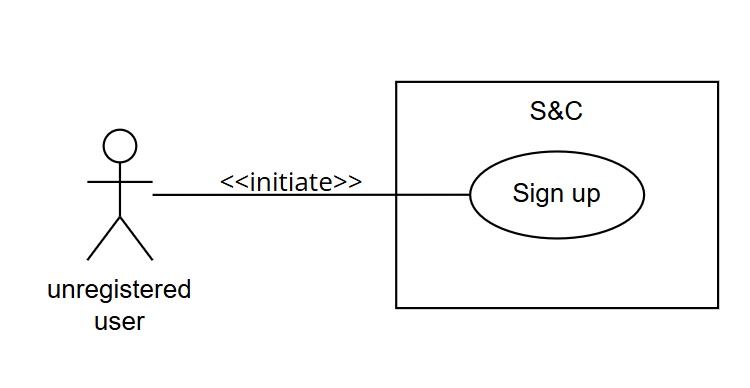
\includegraphics[width=1\linewidth]{Images/use case diagrams/UNREGISTERED_USER.png}
    \caption{Unregistered user use case diagram}
    \label{fig:enter-label}
\end{figure}

\begin{figure}[H]
    \centering
    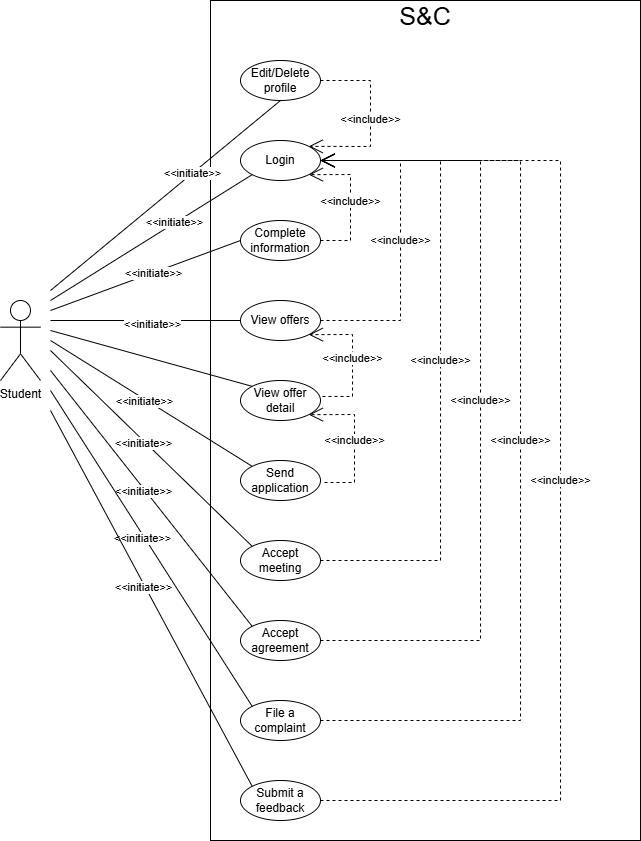
\includegraphics[width=1\linewidth]{Images/use case diagrams/STUDENT.png}
    \caption{Student use case diagram}
    \label{fig:enter-label}
\end{figure}

\begin{figure}[H]
    \centering
    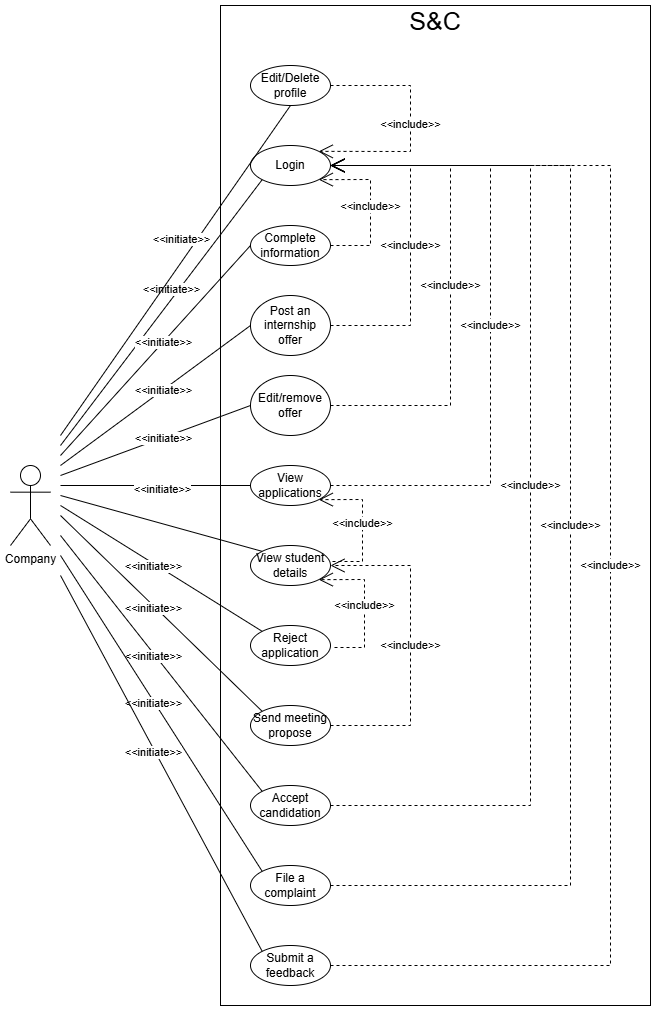
\includegraphics[width=0.9\linewidth]{Images/use case diagrams/COMPANY.png}
    \caption{Company use case diagram}
    \label{fig:enter-label}
\end{figure}

\begin{figure}[H]
    \centering
    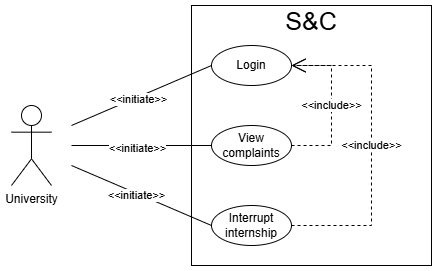
\includegraphics[width=1\linewidth]{Images/use case diagrams/UNIVERSITY.png}
    \caption{University use case diagram}
    \label{fig:enter-label}
\end{figure}

\subsection{Use cases}
\label{subsec: use_cases}%

\newcounter{uc}
\setcounter{uc}{1}
\newcommand{\cuc}{\theuc\stepcounter{uc}}

\textbf{UC\cuc\  - User registration}

\begin{center} 
    \renewcommand{\arraystretch}{1.2} 
    \begin{longtable}{ l p{0.8\linewidth} } 
        \hline 
        Actor & Unregistered User \\ \hline 
        Entry Condition & The user does not have an account and clicks the "Sign Up" button to create a new one. \\ \hline 
        Event Flow & 1.\ The unregistered user opens the S\&C application and clicks the "Sign Up" button. \\ 
        & 2.\ The user fills out all mandatory fields (email, password) and confirms the password. \\ 
        & 3.\ The user agrees to the "Terms \& Conditions" and "Privacy Policy" by checking the corresponding boxes. \\ 
        & 4.\ The user presses the "Sign Up" button to submit the registration form. \\ 
        & 5.\ The S\&C system sends a confirmation email to the provided email address. \\ 
        & 6.\ The user completes the registration by clicking the confirmation link in the email. \\ \hline 
        Exit Condition & The user's account is successfully created, and they can log into the system. \\ \hline 
        Exceptions & 1.\ One or more mandatory fields are empty. \\ 
        & 2.\ An account with the same email already exists. \\ 
        & 3.\ The user has not checked the "Terms \& Conditions" or "Privacy Policy" boxes. \\ \hline 
        \caption{Unregistered User registration process} 
        \label{tab:user_registration_uc} 
    \end{longtable} 
\end{center}

\begin{figure}[H]
    \centering
    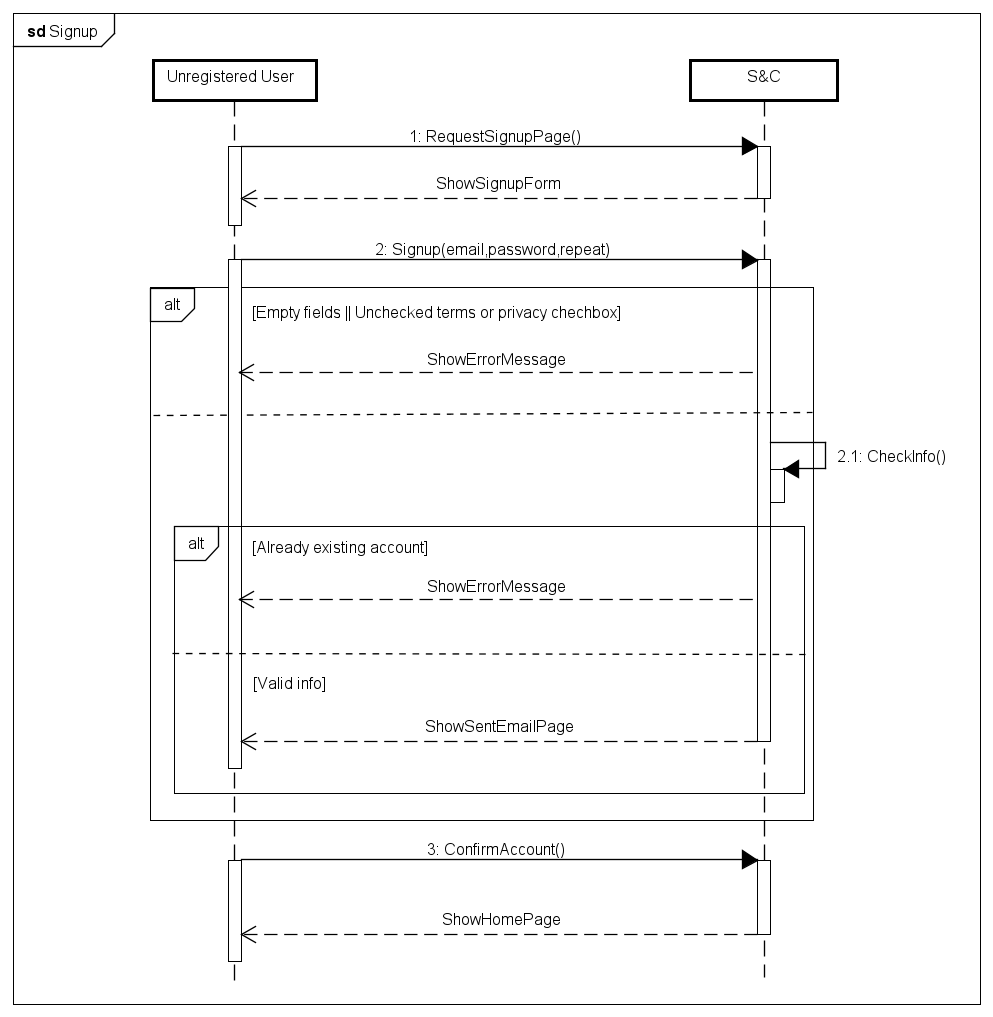
\includegraphics[width=1\linewidth]{Images/Sequence diagrams/Signup.png}
    \caption{User registration sequence diagram}
    \label{fig:enter-label}
\end{figure}

\textbf{UC\cuc\  - User, student, company or university login}

\begin{center}
    \renewcommand{\arraystretch}{1.2} 
    \begin{longtable}{ l p{0.8\linewidth} } 
        \hline
        Actor & Registered user (student, company, or university). \\ \hline
        Entry Condition & A user with an existing account clicks the "Login" button to access the homepage of the S\&C platform. \\ \hline
        Event Flow & 1.\ The user enters their credentials (email, password) in the login form. \\ 
        & 2.\ The user presses the "Login" button. \\ 
        & 3.\ The S\&C system validates the provided credentials. \\ \hline
        Exit Condition & If the credentials are correct, the user is redirected to the homepage. \\ \hline
        Exceptions & 1.\ The provided email is not registered in the platform. \\ 
        & 2.\ The provided password is incorrect. \\ 
        & 3.\ One or both fields (email or password) are left empty. \\ \hline
        \caption{Registered user logs in.}
        \label{tab:goals_tab}%
    \end{longtable}
\end{center}


\begin{figure}[H]
    \centering
    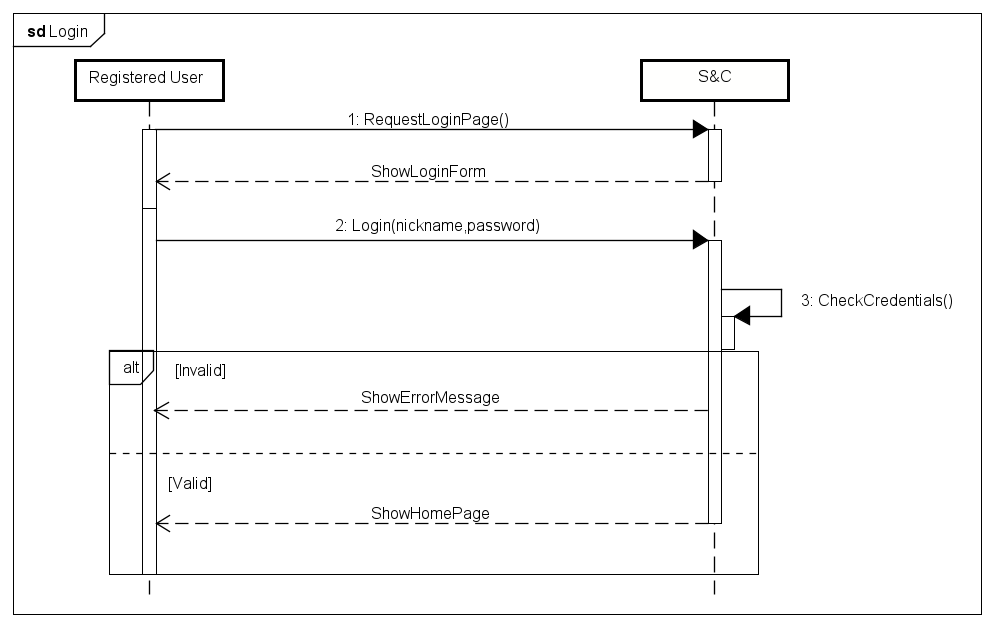
\includegraphics[width=1\linewidth]{Images/Sequence diagrams/Login.png}
    \caption{Login sequence diagram}
    \label{fig:enter-label}
\end{figure}

\textbf{UC\cuc\  - Student's account activation}

\begin{center} 
    \renewcommand{\arraystretch}{1.2} 
    \begin{longtable}{ l p{0.8\linewidth} } 
        \hline 
        Actor & Registered User \\ \hline 
        Entry Condition & The user wants to upgrade their account to a student account to unlock full access to the platform's features. \\ \hline 
        Event Flow & 1.\ The user presses the "Unlock full experience" button on the homepage. \\ 
        & 2.\ The user selects the "Student Account" option. \\  
        & 3.\ The user fills out all mandatory fields (name, surname, academic email, phone number, postal code). \\ 
        & 4.\ The user uploads their CV in PDF format. \\ 
        & 5.\ The user selects their internship goals from a provided checklist. \\ 
        & 6.\ The user presses the "Upgrade Account" button. \\ 
        & 7.\ The system validates the entered information and uploaded CV. \\ 
        & 8.\ If the information is valid, the system sends a confirmation email to verify the academic email's validity. \\ 
        & 9.\ The user clicks on the confirmation link in the email to complete the activation process. \\ \hline 
        Exit Condition & The user's account is successfully upgraded to a student account, granting access to additional features. \\ \hline 
        Exceptions & 1.\ One or more mandatory fields are left empty. \\ 
        & 2.\ The uploaded CV is not in the correct PDF format. \\ 
        & 3.\ The CV file is missing during the upload process. \\ 
        & 4.\ The entered information fails validation checks. \\
        & 5.\ An account with the provided academic email already exists. \\ \hline 
        \caption{User upgrades their account to a Student Account} 
        \label{tab:student_activation_uc} 
    \end{longtable} 
\end{center}

\begin{figure}[H]
    \centering
    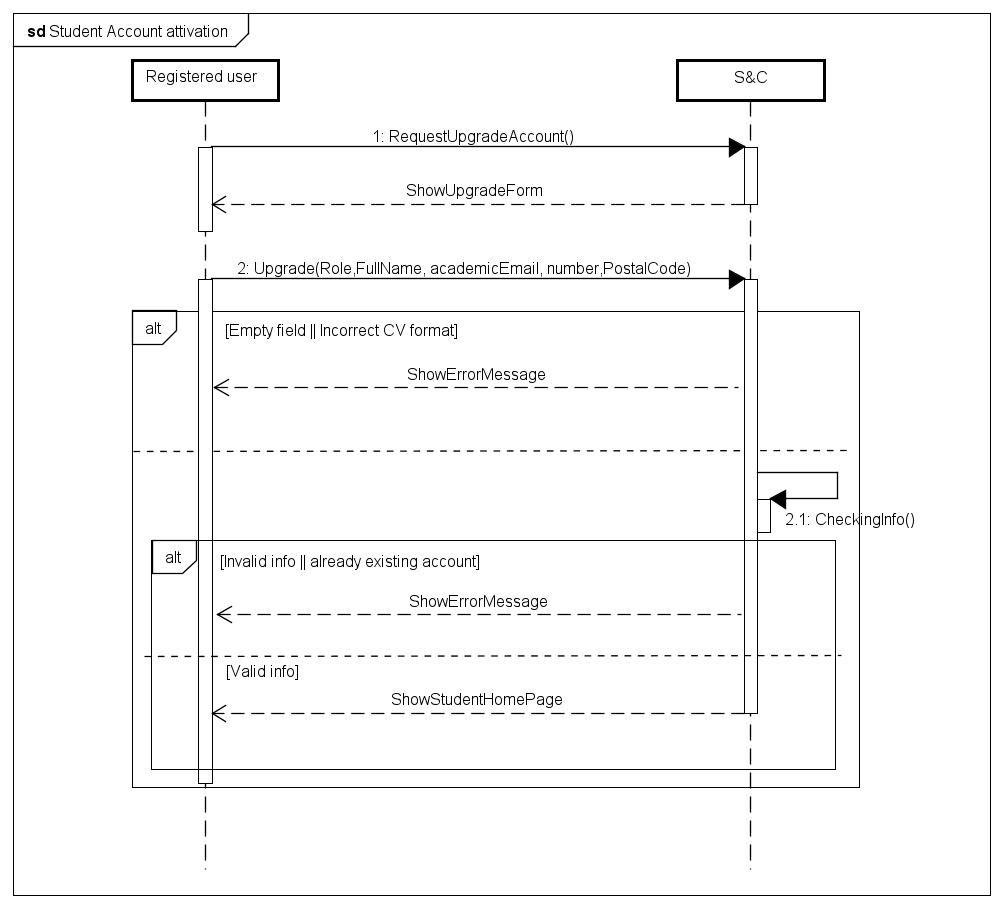
\includegraphics[width=1\linewidth]{Images/Sequence diagrams/Student account attivation.png}
    \caption{Student account activation sequence diagram}
    \label{fig:enter-label}
\end{figure}

\textbf{UC\cuc\  - Student modifies their profile or updates CV.}

\begin{center}
    \renewcommand{\arraystretch}{1.2}
    \begin{longtable}{ l p{0.8\linewidth} } 
        \hline
        Actor & Student \\ \hline
        Entry Condition & The student needs to modify their profile or wants to update their CV. \\ \hline
        Event Flow & 1.\ The student clicks on the "Profile" button. \\
        & 2.\ The student modifies the form with the correct data. \\
        & 2b.\ The student updates their CV with the suggestions offered by the S\&C system to ensure that the system can interpret the included data correctly. \\ 
        & 3.\ The student clicks on the "Update Profile" button. \\ \hline
        Exit Condition & The S\&C system registers the updated data and displays a success message. \\ \hline
        Exceptions & 1.\ One or more mandatory fields are left empty. \\ 
        & 2.\ The uploaded or updated CV is not in the correct PDF format. \\ 
        & 3.\ The entered information fails validation checks. \\ \hline
        \caption{Student updates their profile or CV.}
        \label{tab:student_profile_update_uc}%
    \end{longtable}
\end{center}

\begin{figure}[H]
    \centering
    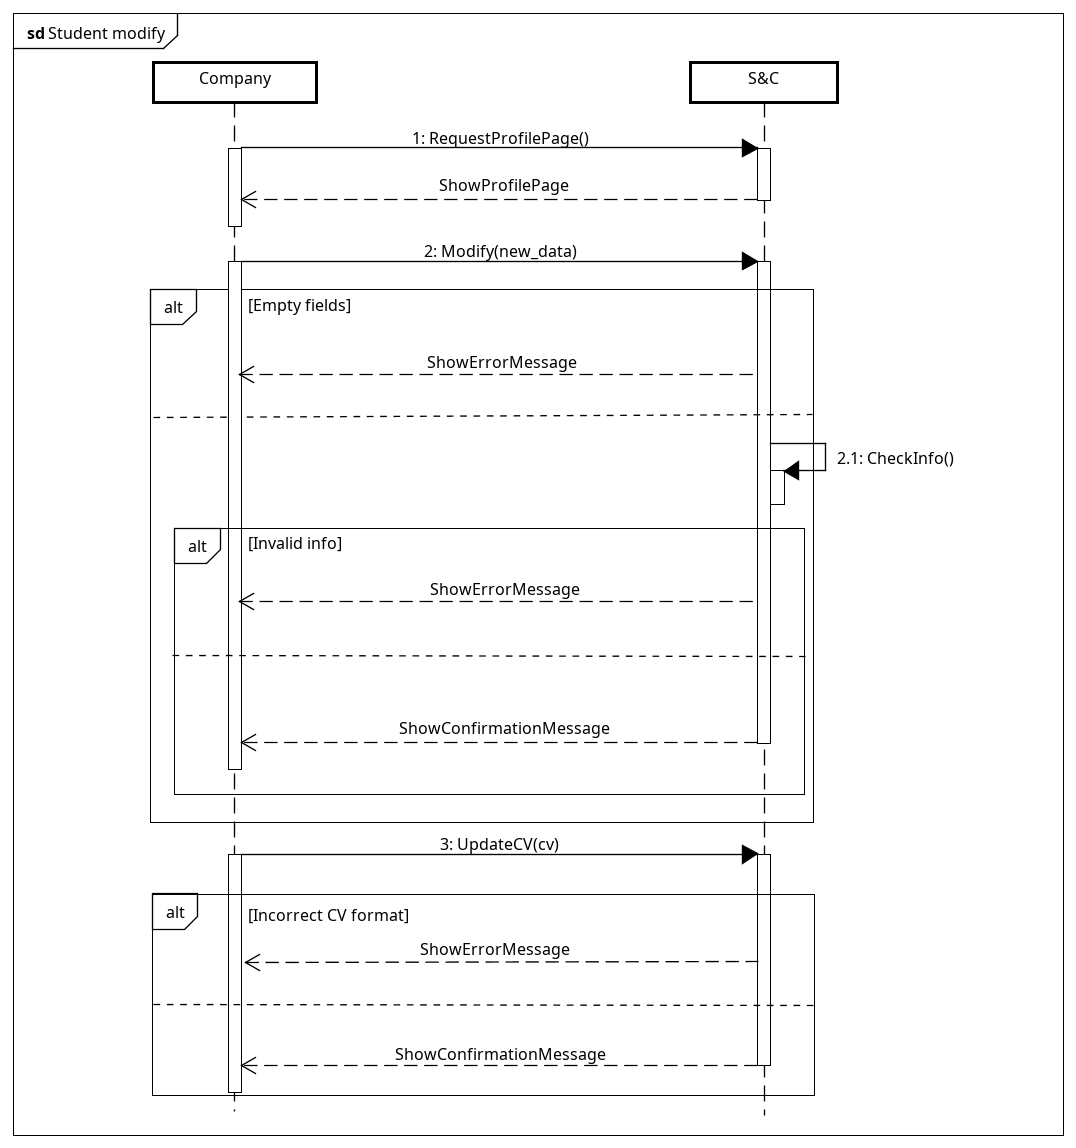
\includegraphics[width=1\linewidth]{Images/Sequence diagrams/Student modify.png}
    \caption{Student's profile update sequence diagram.}
    \label{fig:enter-label}
\end{figure}

\textbf{UC\cuc\  - Student checks available offers.}

\begin{center}
    \renewcommand{\arraystretch}{1.2}
    \begin{longtable}{ l p{0.8\linewidth} } 
        \hline
        Actor & Student \\ \hline
        Entry Condition & 1.\ The student logs in or he student clicks the "Home Page" button. \\ \hline
        Event Flow & 1.\ The student enters the S\&C system by logging in. \\
        & 2.\ If the student is on a different page, they click the "Home Page" button. \\ \hline
        Exit Condition & The S\&C system displays the student's personalized recommended internships. \\ \hline
        Exceptions & System error during page loading or redirection. \\ \hline
        \caption{Student checks available offers.}
        \label{tab:goals_tab}%
    \end{longtable}
\end{center}

\textbf{UC\cuc\  - Student opens details page of an internship post.}

\begin{center}
    \renewcommand{\arraystretch}{1.2}
    \begin{longtable}{ l p{0.8\linewidth} } 
        \hline
        Actor & Student \\ \hline
        Entry condition & Student clicks on the internship post.\\ \hline
        Event Flow       & 1.\ Student enters S\&C system logging in.\\ \hline
        Exit condition & S\&C system redirects shows student their personal recommended internships. \\ \hline
        Exceptions  & System cannot elaborate available internships.
        \\ \hline
        \caption{Student views offers.}
        \label{tab:goals_tab}%
    \end{longtable}
\end{center}

\textbf{UC\cuc\  - Student sends an application for an internship.}

\begin{center} 
    \renewcommand{\arraystretch}{1.2} 
    \begin{longtable}{ l p{0.8\linewidth} } 
        \hline 
        Actor & Student \\ \hline 
        Entry Condition & The student wants to apply for a specific internship offer. \\ \hline 
        Event Flow & 1.\ The student navigates to the internship offer by clicking on its box. \\ 
        & 2.\ The student clicks the "Apply to this internship" button. \\ 
        & 3.\ The system prompts for confirmation, and the student clicks the "Confirm" button to submit the application. \\ \hline 
        Exit Condition & The system displays a success message confirming that the application was submitted. \\ \hline 
        Exceptions & 1.\ The system is unable to process the application due to a technical issue. \\ 
        & 2.\ The internship offer is no longer available. \\ \hline 
        \caption{Student sends an application for an internship} 
        \label{tab:student_application_uc} 
    \end{longtable} 
\end{center}

\begin{figure}[H]
    \centering
    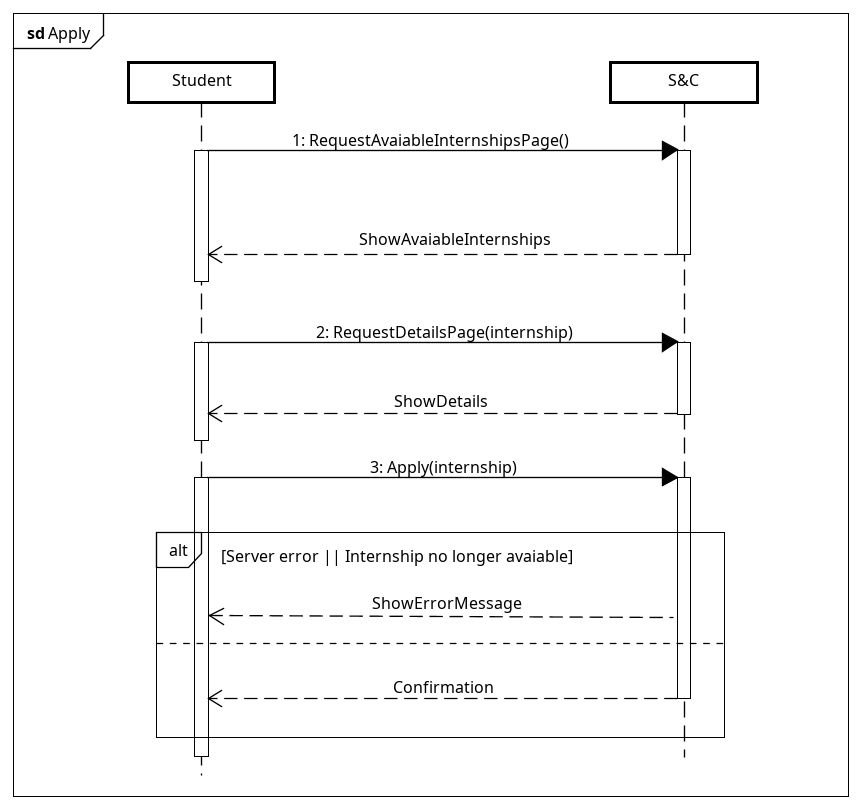
\includegraphics[width=1\linewidth]{Images/Sequence diagrams/Application.png}
    \caption{[UC 5-6-7] Student application sending path sequence diagram}
    \label{fig:enter-label}
\end{figure}

\textbf{UC\cuc\  - Student accepts or denies an interview schedule proposal from the company.}

\begin{center} 
    \renewcommand{\arraystretch}{1.2} 
    \begin{longtable}{ l p{0.8\linewidth} } 
        \hline
        Actor & Student \\ \hline
        Entry Condition & The student receives a notification about an interview schedule proposed by the company. \\ \hline 
        Event Flow & 1.\ The system sends a notification to the student about the interview schedule. \\ 
        & 2.\ The student clicks on the notification, opening a pop-up page displaying the schedule details. \\
        & 3.\ If the student agrees with the schedule, they click the "Accept" button. \\ 
        & 4.\ If the student disagrees, they provide a reason in the designated text field and click the "Deny" button. \\ \hline 
        Exit Condition & The system displays a confirmation message indicating that the student's decision (acceptance or denial) has been successfully registered. \\ \hline 
        Exceptions & 1.\ Schedule Not Available: The company cancels or updates the proposed schedule before the student views it. \\ \hline 
        \caption{Student accepts or denies an interview schedule proposal} 
        \label{tab:student_schedule_uc} 
    \end{longtable} 
\end{center}

\textbf{UC\cuc\  - Student accepts or denies the start of the internship.}

\begin{center} 
    \renewcommand{\arraystretch}{1.2} 
    \begin{longtable}{ l p{0.8\linewidth} } 
        \hline 
        Actor & Student \\ \hline 
        Entry Condition & The student receives a notification about the company's positive decision after the interview process. \\ \hline 
        Event Flow & 1.\ The system notifies the student of the company's decision to offer them the internship. \\ 
        & 2.\ The student clicks on the notification, opening a pop-up page with options to proceed. \\ 
        & 3.\ If the student agrees to start the internship, they click the "Confirm" button. \\ 
        & 4.\ If the student declines the offer, they provide a reason in the designated text field and click the "Deny" button. \\ \hline 
        Exit Condition & The system registers the student's decision (acceptance or denial) and displays a success message confirming the action. \\ \hline 
        \caption{Student Accepts or Denies the Start of an Internship} 
        \label{tab:student_internship_uc} 
    \end{longtable} 
\end{center}

\begin{figure}[H]
    \centering
    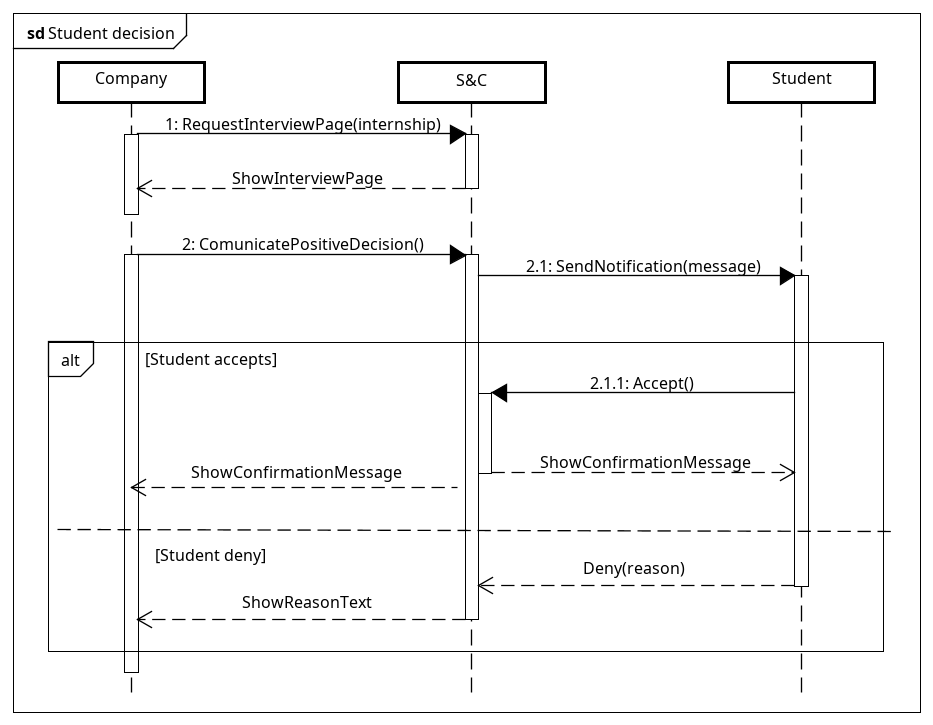
\includegraphics[width=1\linewidth]{Images/Sequence diagrams/Student decision.png}
    \caption{Student's response to internship proposal sequence diagram}
    \label{fig:enter-label}
\end{figure}

\textbf{UC\cuc\  - Company's account activation}

\begin{center} 
    \renewcommand{\arraystretch}{1.2} 
    \begin{longtable}{ l p{0.8\linewidth} } 
        \hline 
        Actor & Registered User \\ \hline 
        Entry Condition & The user wants to upgrade their account to a company account to unlock full access to the platform's features. \\ \hline 
        Event Flow & 1.\ The user presses the "Unlock full experience" button on the homepage. \\ 
        & 2.\ The user selects the "Company Account" option. \\ 
        & 3.\ The user fills in all mandatory fields (full name, phone number, office address). \\ 
        & 4.\ The user presses the "Upgrade Account" button. \\ 
        & 5.\ The system validates the entered information. \\ \hline 
        Exit Condition & The user's account is successfully upgraded to a company account, granting access to additional features. \\ \hline 
        Exceptions & 1.\ One or more mandatory fields are left empty. \\ 
        & 2.\ The entered information fails validation checks. \\ \hline 
        \caption{User upgrades their account to a Company Account} 
        \label{tab:company_activation_uc} 
    \end{longtable} 
\end{center}

\begin{figure}[H]
    \centering
    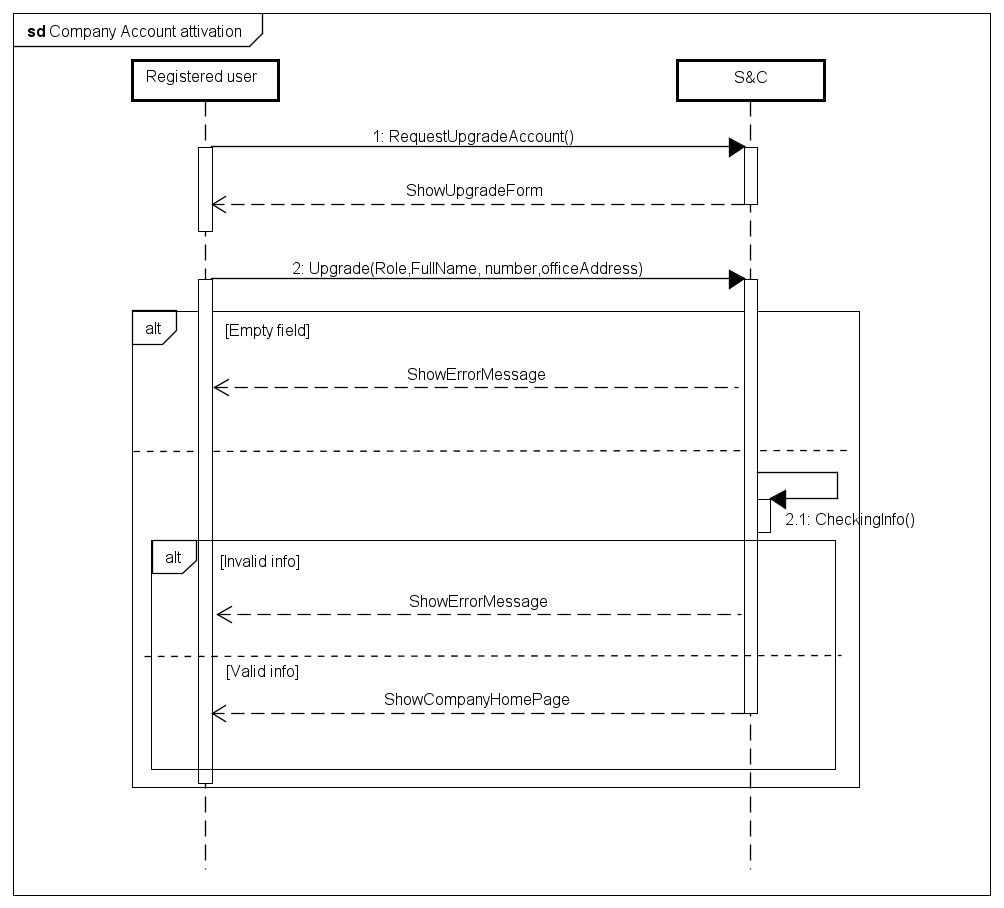
\includegraphics[width=1\linewidth]{Images/Sequence diagrams/Company Account attivation.png}
    \caption{Student account activation sequence diagram}
    \label{fig:enter-label}
\end{figure}

\textbf{UC\cuc\  - Company modifies their profile.}

\begin{center}
    \renewcommand{\arraystretch}{1.2}
    \begin{longtable}{ l p{0.8\linewidth} } 
        \hline
        Actor & Company \\ \hline
        Entry Condition & The company needs to update their profile because some information is incorrect or out of date. \\ \hline
        Event Flow & 1.\ The company clicks on the "Profile" button. \\
        & 2.\ The company modifies the form with the correct data. \\
        & 3.\ The company clicks on the "Update Profile" button. \\ \hline
        Exit Condition & The S\&C system registers the updated data and displays a success message. \\ \hline
        Exceptions & 1.\ One or more mandatory fields are left empty. \\
        & 2.\ The entered information fails validation checks. \\ \hline
        \caption{Company updates their profile.}
        \label{tab:company_profile_update_uc}%
    \end{longtable}
\end{center}

\begin{figure}[H]
    \centering
    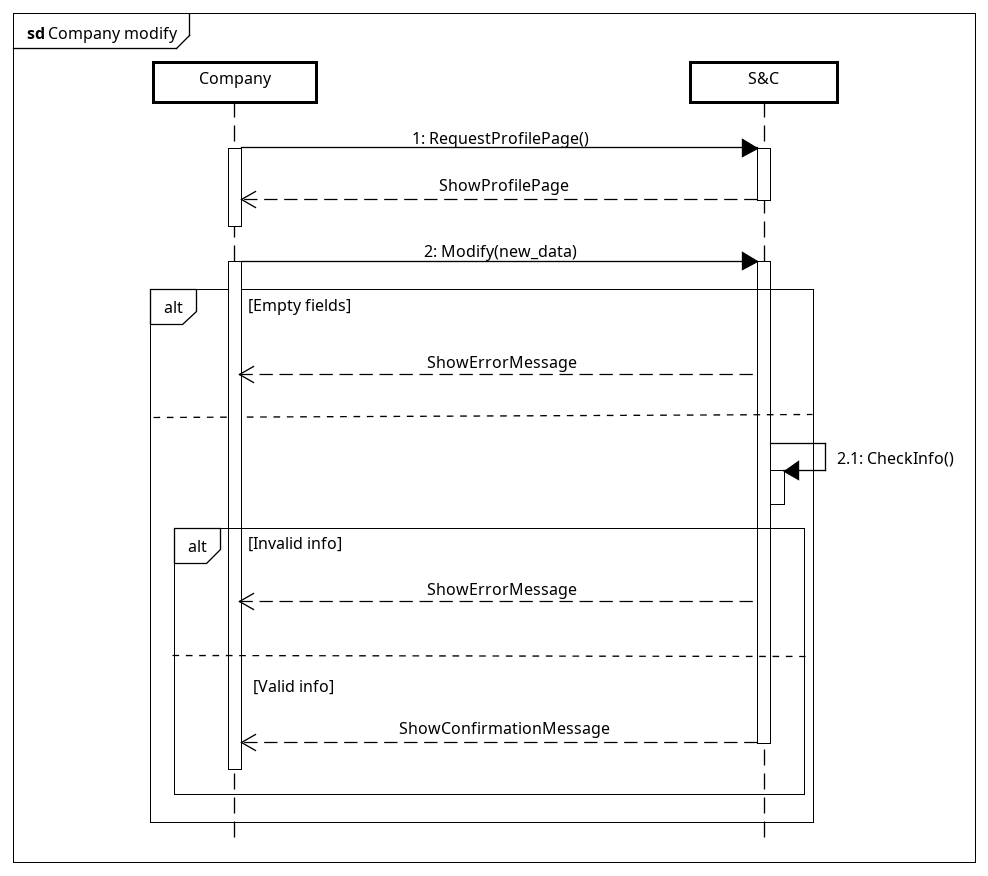
\includegraphics[width=1\linewidth]{Images/Sequence diagrams/Company modify.png}
    \caption{Company's profile update sequence diagram}
    \label{fig:enter-label}
\end{figure}

\textbf{UC\cuc\  - Company posts a new internship offer}

\begin{center} 
    \renewcommand{\arraystretch}{1.2} 
    \begin{longtable}{ l p{0.8\linewidth} } 
        \hline 
        Actor & Company \\ \hline 
        Entry Condition & The company decides to create and publish a new internship offer to attract suitable candidates. \\ \hline Event Flow & 1.\ The company presses the "+" button on the homepage. \\ 
        & 2.\ The company fills out the internship offer form, inserting project description, requested role, location address (if different from the default office address), salary (if applicable), number of students (if more than one is required), skills the student will gain, weekly schedule, benefits offered as mentorship, training opportunities, etc. This process is assisted by system-generated suggestions designed to make the post more appealing and engaging for students \\ 
        & 3.\ The company reviews the information and clicks the "Post offer" button. \\ \hline 
        Exit Condition & The system successfully registers the new internship offer and displays a confirmation message. The offer becomes visible to students. \\ \hline 
        Exceptions & 1.\ One or more mandatory fields in the form are left empty.\\ \hline 
        \caption{Company posts a new internship offer} 
        \label{tab:company_post_offer_uc} 
    \end{longtable} 
\end{center}

\begin{figure}[H]
    \centering
    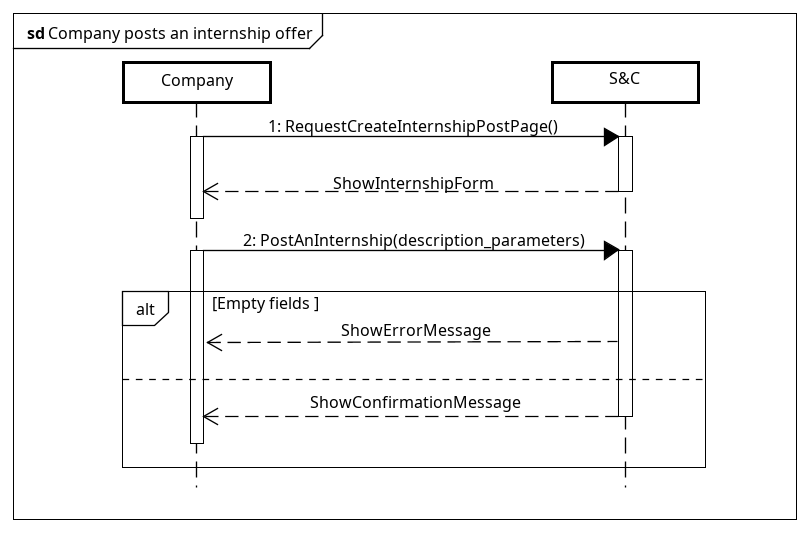
\includegraphics[width=1\linewidth]{Images/Sequence diagrams/Company posts an internship offer.png}
    \caption{Company internship post creation sequence diagram}
    \label{fig:enter-label}
\end{figure}

\textbf{UC\cuc\  - The company accepts an application or identifies a promising student and proposes a schedule for the interview}

\begin{center} 
    \renewcommand{\arraystretch}{1.2} 
    \begin{longtable}{ l p{0.8\linewidth} } 
        \hline 
        Actor & Company \\ \hline 
        Entry Condition & 1.\ The company is notified about a new application from a suitable student. \\ 
        & 2.\ The company decides to accept an application from a student. \\ 
        & 3.\ The company identifies a promising student directly from the system, even if the student has not sent an application. \\ \hline 
        Event Flow &  1.\ The company clicks on the notification received about a matching student's application. \\
        & 1b.\ Alternatively, the company navigates to the internship offer, clicks on the its box and selects the student's profile. \\ 
        & 1c.\ As another option, the company searches for the student’s profile from the internship offer and selects it. \\ 
        & 2.\ The system displays the student’s detailed profile page. \\ 
        & 3.\ The company clicks the "Propose interview" or "Contact student" button. \\ 
        & 4.\ A pop-up form appears, allowing the company to schedule an interview. \\ 
        & 5.\ The company completes the form with details such as date and time of the interview, format (in-person, video call), additional comments or instructions (if any). \\ 
        & 6.\ The company clicks the "Send proposal" button. \\ \hline 
        Exit Condition & The system successfully registers the interview proposal and notifies the student. A confirmation message is displayed to the company. \\ \hline 
        Exceptions & 1.\ One or more mandatory fields in the interview scheduling form are left empty. \\ 
        & 2.\ The student is already engaged in another internship or is unavailable. \\ \hline
        \caption{The company accepts an application or identifies a promising student and proposes a schedule for the interview} 
        \label{tab:company_post_offer_uc} 
    \end{longtable} 
\end{center}

\begin{figure}[H]
    \centering
    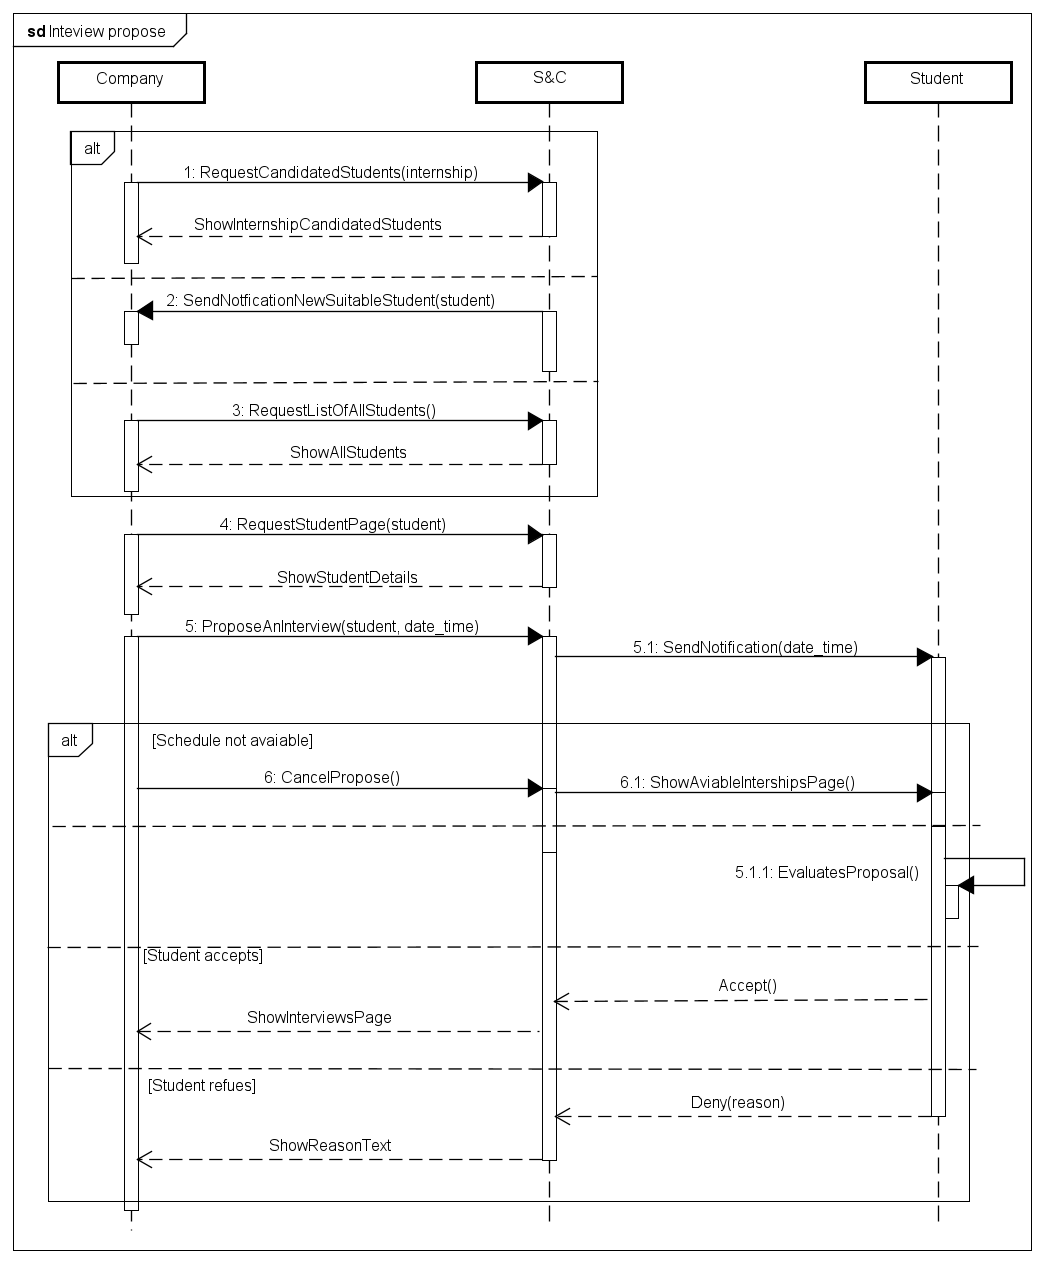
\includegraphics[width=1\linewidth]{Images/Sequence diagrams/Inteview propose.png}
    \caption{[UC 8-13] Interview propose path sequence diagram}
    \label{fig:enter-label}
\end{figure}

\textbf{UC\cuc\  - Student or Company submits a complaint about an ongoing internship.}

\begin{center} 
    \renewcommand{\arraystretch}{1.2} 
    \begin{longtable}{ l p{0.8\linewidth} } 
        \hline Actor & Student or Company \\ \hline 
        Entry Condition & The actor identifies a problem or negative aspect of their ongoing internship and wants to notify the university. \\ \hline 
        Event Flow & 1.\ The actor navigates to the "ongoing internship" tab. \\  
        & 2.\ The actor fills out the complaint form, providing details about the issue. \\ 
        & 3.\ The actor clicks the "Submit" button to send the complaint. \\ \hline 
        Exit Condition & The system successfully registers the complaint and confirms its submission to the university. \\ \hline
        \caption{Student or Company submits a complaint about an ongoing internship} 
        \label{tab:student_complaint_uc} 
    \end{longtable} 
\end{center}

\begin{figure}[H]
    \centering
    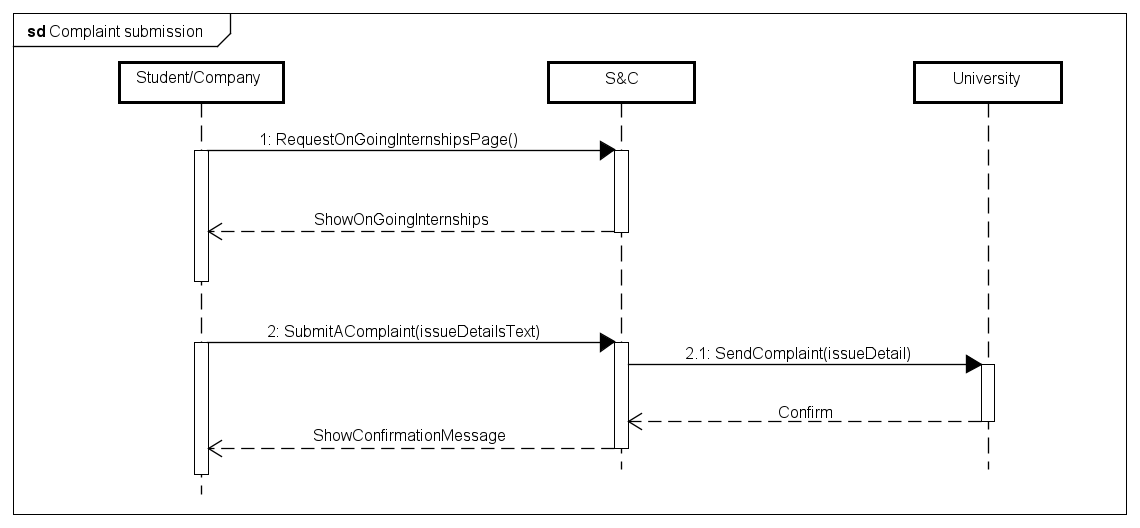
\includegraphics[width=1\linewidth]{Images/Sequence diagrams/Complaint submission.png}
    \caption{Student/Company complaint submission sequence diagram}
    \label{fig:enter-label}
\end{figure}

\textbf{UC\cuc\  - Student or Company submits a feedback about a terminated internship.}

\begin{center} 
    \renewcommand{\arraystretch}{1.2} 
    \begin{longtable}{ l p{0.8\linewidth} } 
        \hline 
        Actor & Student or Company \\ \hline 
        Entry Condition & The internship has been terminated and an actor wants to provide feedback to help improve the system's recommendations. \\ \hline 
        Event Flow & 1.\ The actor navigates to the "terminated internships" section. \\
        & 2.\ The actor selects the relevant internship from the list. \\
        & 3.\ The actor fills out the feedback form, providing details about their experience, including pros, cons, and suggestions. \\
        & 4.\ The actor clicks the "Submit feedback" button to send it. \\ \hline 
        Exit Condition & The system successfully registers the actor's feedback, which is used to refine the recommendation algorithm and enhance future matches. \\ \hline  
        \caption{Student or Company submits feedback about a terminated internship} 
        \label{tab:student_feedback_uc} 
    \end{longtable} 
\end{center}

\begin{figure}[H]
    \centering
    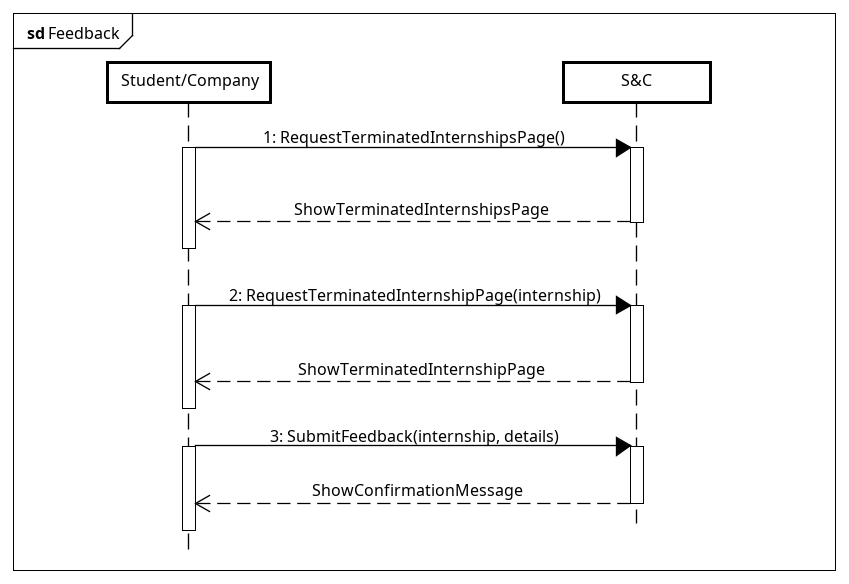
\includegraphics[width=1\linewidth]{Images/Sequence diagrams/Feedback.png}
    \caption{Student/Company feedback submission sequence diagram}
    \label{fig:enter-label}
\end{figure}

\textbf{UC\cuc\  - University decides to interrupt an internship due to relevant complaints.}

\begin{center} 
    \renewcommand{\arraystretch}{1.2} 
    \begin{longtable}{ l p{0.8\linewidth} } 
        \hline 
        Actor & University \\ \hline 
        Entry Condition & 1.\ The university is notified about a complaint concerning an ongoing internship. \\ 
        & 2.\ The university determines that the issue reported is significant enough to warrant the termination of the internship. \\ \hline
        Event Flow &  1.\ The university clicks on the notification related to the complaint. \\ 
        & 1b.\ Alternatively, the university navigates to the "Current internships" list and selects the internship. \\ 
        & 2.\ The system displays the details of the internship and the associated complaint(s). \\ 
        & 3.\ The university clicks the "Interrupt internship" button. \\ 
        & 4.\ A confirmation pop-up appears, and the university provides a reason for the interruption in a text field. \\ 
        & 5.\ The university clicks "Confirm" to finalize the decision. \\ \hline 
        Exit Condition & The system successfully registers the decision and sends notifications to both the company and the student, detailing the reason for the termination. \\ \hline
        \caption{University Decides to Interrupt an Internship Due to Relevant Complaints} 
        \label{tab:university_interrupt_uc} 
    \end{longtable} 
\end{center}

\begin{figure}[H]
    \centering
    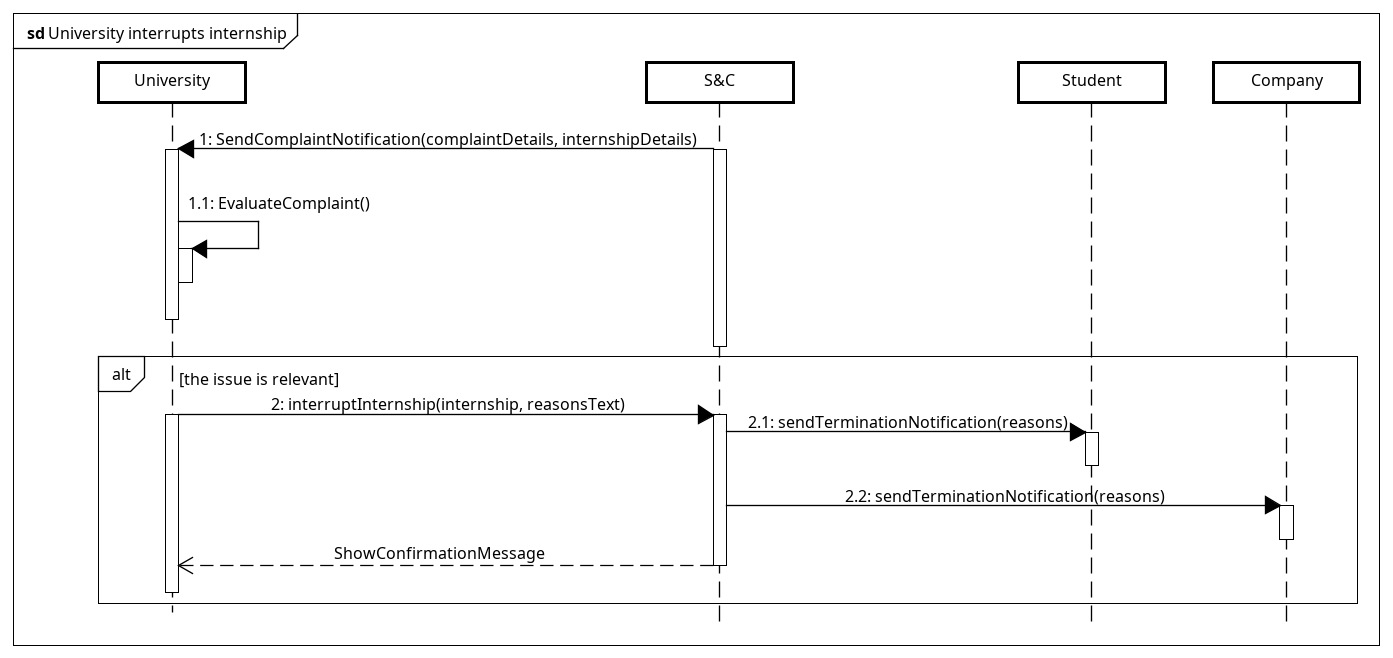
\includegraphics[width=1\linewidth]{Images/Sequence diagrams/University interrupts internship.png}
    \caption{University internship interrupt sequence diagram}
    \label{fig:enter-label}
\end{figure}


\clearpage

\subsection{Mapping on goals}
\label{subsec: map_on_g}%

\begin{itemize}
    \item \textbf{G1 - Allows Companies to advertise their internship offers to find the most suitable students, with the help of recommendation.}
    \begin{itemize}
        \item R1: S\&C system allows unregistered users to sign-up.
        \item R2: S\&C system allows registered users to verify their email address.
        \item R6: S\&C system allows registered users to view posted internships on the platform.
        \item R27: S\&C system allows Companies to post internship offers by providing detailed information.
        \item R28: S\&C system allows Companies to edit an internship's post.
        \item R29: S\&C system allows Companies to delete an internship's post.
        \item R30: S\&C system allows Companies to identify the most suitable students on the platform for their internship posts, even if the students have not applied.
        \item R47: S\&C system periodically updates internship recommendations based on new data from Students and Companies.
    \end{itemize}
    \item \textbf{G2 - Allows Students to look for internships based on their needs and find the most suitable for them, with the help of recommendation.}
    \begin{itemize}
        \item R4: S\&C system allows registered users to edit their account details.
        \item R7: S\&C system allows registered users to upgrade to a Student account or a Company account.
        \item R9: S\&C system allows registered users to update their notifications preferences.
        \item R10: S\&C system allows Students to view a personalized dashboard in their homepage.
        \item R11: S\&C system allows Students to explore available internships.
        \item R12: S\&C system allows Students to view available internships ordered by the best matching, based on a matching score system.
        \item R13: S\&C system allows Students to change the default order.
        \item R14: S\&C system allows Students to apply filters on the view of the available internships.
        \item R15: S\&C system allows Students to receive notification when a new internship matching their profile is posted.
        \item R16: S\&C system allows Students to view the details of a specific internship page.
        \item R33: S\&C system allows Companies to receive notification when a new student with a high matching score has applied.
        \item R46: S\&C system improves recommendation accuracy by considering user feedback on previous internships.
        \item R47: S\&C system periodically updates internship recommendations based on new data from Students and Companies.
    \end{itemize}
    \item \textbf{G3 - Supports selection process by helping manage interviews and also finalize the selections.}
    \begin{itemize}
        \item R17: S\&C system allows Students to apply for an internship.
        \item R18: S\&C system allows Students to view sent applications.
        \item R19: S\&C system allows Students to monitor the status of an application.
        \item R20: S\&C system allows Students to withdraw a sent application.
        \item R21: S\&C system allows Students to confirm their participation of a scheduled interview via a notification interface.
        \item R22: S\&C system allows Students to decline an interview offer via a notification interface.
        \item R31: S\&C system allows Companies to review the applications for an internship.
        \item R32: S\&C system allows Companies to view internship's applications ordered by the best match.
        \item R34: S\&C system allows Companies to propose a date to a student to schedule an interview.
        \item R35: S\&C system allows Companies to prepare a standardized set of questions to be proposed to all candidates for a specific internship.
        \item R36: S\&C system allows Companies to compare the answers from all candidates to facilitate the selection process.
        \item R37: S\&C system allows Companies to reject a student after the interview.
    \end{itemize}
    \item \textbf{G4 - Provides suggestions to companies regarding how to make their offers more appealing for students.}
    \begin{itemize}
        \item R27: S\&C system allows Companies to post internship offers by providing detailed information.
        \item R46: S\&C system improves recommendation accuracy by considering user feedback on previous internships.
    \end{itemize}
    \item \textbf{G5 - Provides suggestions to students how to make their CVs more appealing for companies.}
    \begin{itemize}
        \item R8: S\&C system allows registered users to verify their current academic status by validating their institutional email address.
        \item R24: S\&C system allows Students to review the agreements of an internship before accepting.
    \end{itemize}
    \item \textbf{G6 - Allows stakeholders to monitor the progress of internships, report issues, and track outcomes.}
    \begin{itemize}
        \item R5: S\&C system allows registered users to delete their account.
        \item R23: S\&C system sends automated reminders to Students for upcoming interview deadlines.
        \item R26: S\&C system allows Students to submit feedback after completing an internship.
        \item R38: S\&C system allows Companies to start an internship.
        \item R39: S\&C system allows Companies to view active internships.
        \item R40: S\&C system allows Companies to file a complaint.
        \item R41: S\&C system allows Companies to submit feedback after completing an internship.
        \item R43: S\&C system allows universities to collect complaints raised by Students.
        \item R44: S\&C system allows universities to collect complaints raised by Companies.
    \end{itemize}

    
    \item \textbf{G7 - Allows Universities to monitor the situation of ongoing internships and interrupt them when necessary.}
    \begin{itemize}
        \item R3: S\&C system allows registered users to login.
        \item R25: S\&C system allows Students to file a complaint.
        \item R42: S\&C system allows universities to login to the system providing credentials.
        \item R45: S\&C system allows universities to mediate between Student and Company after a complaint.
    \end{itemize}
\end{itemize}

\clearpage

\renewcommand{\arraystretch}{1.5}
    \begin{longtable}{|l|c|c|c|c|c|c|c|}
        \hline
        \textbf{Requirement} & \textbf{G1} & \textbf{G2} & \textbf{G3} & \textbf{G4} & \textbf{G5} & \textbf{G6} & \textbf{G7} \\
        \hline
            R1  & \checkmark &   &   &   &   &   &   \\ \hline
            R2  & \checkmark &   &   &   &   &   &   \\ \hline
            R3  &   &   &   &   &   &   & \checkmark \\ \hline
            R4  &   & \checkmark &   &   &   &   &   \\ \hline
            R5  &   &   &   &   &   & \checkmark &   \\ \hline
            R6  & \checkmark &   &   &   &   &   &   \\ \hline
            R7  &   & \checkmark &   &   &   &   &   \\ \hline
            R8  &   &   &   &   & \checkmark &   &   \\ \hline
            R9  &   & \checkmark &   &   &   &   &   \\ \hline
            R10 &   & \checkmark &   &   &   &   &   \\ \hline
            R11 &   & \checkmark &   &   &   &   &   \\ \hline
            R12 &   & \checkmark &   &   &   &   &   \\ \hline
            R13 &   & \checkmark &   &   &   &   &   \\ \hline
            R14 &   & \checkmark &   &   &   &   &   \\ \hline
            R15 &   & \checkmark &   &   &   &   &   \\ \hline
            R16 &   & \checkmark &   &   &   &   &   \\ \hline
            R17 &   &   & \checkmark &   &   &   &   \\ \hline
            R18 &   &   & \checkmark &   &   &   &   \\ \hline
            R19 &   &   & \checkmark &   &   &   &   \\ \hline
            R20 &   &   & \checkmark &   &   &   &   \\ \hline
            R21 &   &   & \checkmark &   &   &   &   \\ \hline
            R22 &   &   & \checkmark &   &   &   &   \\ \hline
            R23 &   &   &   &   &   & \checkmark &   \\ \hline
            R24 &   &   &   &   & \checkmark &   &   \\ \hline
            R25 &   &   &   &   &   &   & \checkmark \\ \hline
            R26 &   &   &   &   &   & \checkmark &   \\ \hline
            R27 & \checkmark &   &   & \checkmark &   &   &   \\ \hline
            R28 & \checkmark &   &   &   &   &   &   \\ \hline
            R29 & \checkmark &   &   &   &   &   &   \\ \hline
            R30 & \checkmark &   &   &   &   &   &   \\ \hline
            R31 &   &   & \checkmark &   &   &   &   \\ \hline
            R32 &   &   & \checkmark &   &   &   &   \\ \hline
            R33 &   & \checkmark &   &   &   &   &   \\ \hline
            R34 &   &   & \checkmark &   &   &   &   \\ \hline
            R35 &   &   & \checkmark &   &   &   &   \\ \hline
            R36 &   &   & \checkmark &   &   &   &   \\ \hline
            R37 &   &   & \checkmark &   &   &   &   \\ \hline
            R38 &   &   &   &   &   & \checkmark &   \\ \hline
            R39 &   &   &   &   &   & \checkmark &   \\ \hline
            R40 &   &   &   &   &   & \checkmark &   \\ \hline
            R41 &   &   &   &   &   & \checkmark &   \\ \hline
            R42 &   &   &   &   &   &   & \checkmark \\ \hline
            R43 &   &   &   &   &   & \checkmark &   \\ \hline
            R44 &   &   &   &   &   & \checkmark &   \\ \hline
            R45 &   &   &   &   &   &   & \checkmark \\ \hline
            R46 &   & \checkmark &   & \checkmark &   &   &   \\ \hline
            R47 & \checkmark & \checkmark &   &   &   &   &   \\ \hline
        \caption{ Traceability Matrix for Goals and Requirements}
    \end{longtable}
\label{tab:mapping_requirements}



\section{Performance Requirements}
\label{sec:performance_requirements}%
The platform has to guarantee good performances in order to work efficiently and correctly for a great number of users (Universities, Students and Companies). In order to achieve this the response time must be lower than a second, this is due to the fact that the user's connection to the platform can be slow and the loading times can subsequently increase in an exponential way.

\section{Design Constraints}
\label{sec:performance_requirements}%

\subsection{Standard compliance}
\label{subsec: standard_compliance}%
The S\&C platform adheres to regulations and standards to ensure data privacy and usability. It complies with the General Data Protection Regulation (GDPR) for secure handling of personal data, including student CVs and company profiles. Additionally, all communications use HTTPS to guarantee secure data transmission, and the international format for date and time is adopted to ensure clarity and consistency across different regions. 
\subsection{Hardware limitations}
\label{subsec: hardware_limitations}%
Here we have a short list of the hardware features that a user should have to use the platform without encountering major problems:
\begin{itemize}
    \item The user must have a device with a good internet connection this means that the device in question should be compatible with at least one of the following standards : 3G, 4G, 5G, IEEE 802.11 or IEEE 802.3. Both wired and wireless connections must be guaranteed during the usage of the platform.
    \item The user must have a device with good hardware features such as a processor with high performance 
\end{itemize}
 
\subsection{Any Other Constraint}
\label{subsec: hardware_limitations}%
In a way, the system ought to give top priority to how user-friendly it is, providing interfaces that feel easy to learn for students, companies, and universities alike for things like uploading resumes, handling internships, and sorting out complaints. It must integrate efficiently with third-party tools (e.g., video conferencing softwares) and ensure compatibility with APIs that support future features (e.g. AI-based recommendations).  The architecture must be as scalable as the platform itself increases in the number of users. The platform should also be integrated with specific tools in order to make the feedback and complaint system robust.
\section{Software system attributes}
\label{sec:performance_requirements}%

\subsection{Reliability}
\label{subsec: reliability}%
The system has to be reliable since it will have to run without stopping for a long period of time. To ensure this feature the platform must have some sort of replication and consistency policy to avoid system crash. In addition to this it is a good practice to have offline backups of the system for recovering information in case of data loss. 
\subsection{Availability}
\label{subsec: availability}%
The system must guarantee an availability of 99\% to support its users effectively, especially during peak usage periods like internship deadlines or videoconferencing sessions. To achieve this, single points of failure must be avoided and load balancing techniques should be used. 
\subsection{Security}
\label{subsec: security }%
User data, including personal information and CVs, must be protected using encryption methods for stored data and secure transmission protocols. The platform must implement measures to prevent unauthorized access and ensure the integrity and confidentiality of user information. 
\subsection{Maintainability}
\label{subsec: maintainability}%
The system must be easily maintainable with well-documented code and routine testing procedures. At least 75\% of the code, excluding the UI, must have test coverage to facilitate debugging and future development and expansion of the platform. 
\subsection{Portability}
\label{subsec: portability}%
As a web-based application, the platform must work correctly on various devices and browsers, such as Chrome, Firefox, and Safari. Compatibility with both desktop and mobile devices ensures usability for a wide range of users. 